\documentclass[12pt]{article}

\usepackage[utf8]{inputenc}
\usepackage[margin=0.6in]{geometry}

\usepackage{amsmath}
\usepackage{graphicx}
\usepackage{booktabs}

\newcommand{\D}[2]{\frac{\mathrm{d}#1}{\mathrm{d}#2}}
\newcommand{\pfrac}[2]{\left(\frac{#1}{#2} \right)}
\newcommand{\ex}[1]{\left\langle#1\right\rangle}

\newcommand{\pdiff}[2]{\frac{\partial#1}{\partial#2}}

\begin{document}

\section{Relative Velocity of Maxwell Boltzmann Gases}

Let's consider the joint probability for the velocities of one particle from each population:

\[ p(v_1,v_2) = \pfrac{\sqrt{m_1 m_2}}{2\pi kT}^3 e^{-(m_1 v_1^2 + m_2 v_2^2) / 2kT} d^3 v_1 d^3 v_2
\]

We can change variables to their center of mass velocity, \(V\) and relative velocity, \(v\), so that now

\begin{align*}
v_1 &= V + \frac{m_2}{M}v\\
v_2 &= V - \frac{m_1}{M}v\\
 p(v_1,v_2) &= \pfrac{\sqrt{m_1 m_2}}{2\pi kT}^3 e^{-(MV^2 + \mu v^2) / 2kT} d^3 v_1 d^3 v_2
\end{align*}

where \(M = m_1 + m_2\) and \(\mu\) is the reduced mass. Next we need to find the Jacobian Determinant of this transformation. Notice that it can be written in block matrix form as

\[ J = \left|  \begin{array}{cc} 
	\pdiff{v_1}{V} & \pdiff{v_2}{V} \\[11pt]
	\pdiff{v_1}{v} & \pdiff{v_2}{v}

\end{array} \right|
\]

where
\[ \pdiff{v_1}{V} = \left(\begin{array}{ccc}
	\pdiff{v_{1x}}{V_x} & \pdiff{v_{1y}}{V_x} & \pdiff{v_{1z}}{V_x} \\
	\pdiff{v_{1x}}{V_y} & \ddots &  \\
	\vdots & & \ddots
	
\end{array}\right)
\]\\

and so on. We can evaluate each block to get \\

\[ J = \left|  \begin{array}{cc} 
	I & I \\[11pt]
	\frac{m_2}{M}I & -\frac{m_1}{M}I 
\end{array} \right|
\]\\

Apparently, the algebra of block matrix determinants is fairly complicated in the general case, but there's a nice result for \(2\times 2\) matrices of square blocks:

\[ J = \left|  -\frac{m_1}{M}I^2 - \frac{m_2}{M}I^2 \right| = \left| -I\right| = (-1)^3 = -1
\]\\

So \(d^3 v_1 d^3 v_2 = d^3 V d^3 v\) and we can write

\[ p(V,v) = \pfrac{\sqrt{m_1 m_2}}{2\pi kT}^3 e^{-(MV^2 + \mu v^2) / 2kT} d^3 V d^3 v
\]

We can get just \(p(v)\) now by marginalizing over \(V\):

\begin{align*}
p(v) &= \int_V  p(V,v) d^3 V d^3 v \\[11pt]
&=\pfrac{\sqrt{m_1 m_2}}{2\pi kT}^3 \iiint dV_x dV_y dV_z e^{-\mu v^2 / 2kT} e^{-MV_x^2/2kT}e^{-MV_x^2/2kT}e^{-MV_x^2/2kT} d^3 v \\[11pt]
&=\pfrac{\sqrt{m_1 m_2}}{2\pi kT}^3  \pfrac{2\pi kT}{M}^{3/2} e^{-\mu v^2 / 2kT} d^3v \\[11pt]
&= \pfrac{\mu}{2\pi kT}^{3/2} e^{-\mu v^2 / 2kT} d^3v
\end{align*}

\section{Nuclear Reaction Chains and Abundances}

\subsection{}

\newcommand{\nc}[2]{n_{^{#1}\mathrm{#2}}}
\newcommand{\dnc}[2]{\dot{n}_{^{#1}\mathrm{#2}}}

Let \(r_i\) be the reaction rate for the \(i^{\mathrm{ith}}\) reaction in the PPI chain.

\begin{align*}
r_1 &= \frac{1}{2}\lambda_1 \nc{1}{H}^2 \\
r_2 &= \lambda_2 \nc{1}{H}\nc{2}{H} \\
r_3 &= \frac{1}{2}\lambda_3 \nc{3}{He}^2
\end{align*}

We have

\begin{align*}
\dnc{1}{H} &= -2r_1 - r_2 + 2r_3 \\
\dnc{2}{H} &= r_1 - r_2\\
\dnc{3}{He} &= -2r_3 + r_2 \\
\dnc{4}{He} &= r_3
\end{align*}

Since the \(r_i\) can be computed from the \(n_i\), this is enough to determine the trajectory of the system, but we do have a fifth equation, \(\dnc{1}{H} + \dnc{2}{H} +\dnc{3}{He} +\dnc{4}{He} = 0\)

\subsection{}

We can take \(r_1 = r_2\) to find \(  \frac{\nc{2}{H}}{\nc{1}{H}} = \frac{\lambda_1}{2\lambda_2} = \pfrac{\tau_1}{\tau_2}^2\frac{S_1}{2S_2}e^{-(\tau_1+\tau_2)/kT}\). Using the expression for \(\tau\) from the lecture notes, \(3 \times 1.22(Z_1^2 Z_2^2 \bar{A} T_6^2)^{1/3}/kT \) yields numerical overflow. Clearly, I'm getting the wrong formula, but time was already short a few days ago.

\section{He flash}

Keeping density and helium concentration constant, we're left with a pretty simple differential equation to step through. This is implemented in the attached notebook with a simple euler integrator.

\includegraphics[scale=.4]{he_flash1.png}
\includegraphics[scale=.4]{he_flash2.png}

We can see the helium flash taking about 490 days to start. I spent some time thinking about how to evaluate whether or not this is a reasonable timescale, but the runaway triple alpha reaction does make intuitive sense; if the star is highly degenerate, its density    only weakly varies with temperature, and cannot cool by expansion, so we expect a degenerate star to warm up. If it also happens that triple alpha process power output increases with temperature in this regime, we expect positive temperature feedback to quickly heat the star to the point that it is no longer degenerate.




\section{Nuclear Statistical Equilibrium}
\subsection{}

Following the prescription, we take \(g_i = 1\) and solve for \(\mu_i\):

\[ \mu_i = m_i c^2 + kT \log{n_i} - \frac{3}{2}kT\log{\frac{m_i kT}{2\pi\hbar^2}}
\]


\newcommand{\muhe}{\mu_{\mathrm{He}}}
\newcommand{\muni}{\mu_{\mathrm{Ni}}}
\newcommand{\mhe}{m_{\mathrm{He}}}
\newcommand{\mni}{m_{\mathrm{Ni}}}
\newcommand{\nhe}{n_{\mathrm{He}}}
\newcommand{\nni}{n_{\mathrm{Ni}}}

Setting \(14\muhe = \muni\),
\[
\frac{\nhe^{14}}{\nni} = \pfrac{\mni kT}{2\pi\hbar^2}^{-\frac{3}{2}}\pfrac{\mhe kT}{2\pi\hbar^2}^{21} e^{(\mni-14\mhe)c^2/kT}
\]

\subsection{}

\( n = \rho X / m  \) so that the above becomes

\begin{align*}
\frac{X_{4}^{14}}{X_{56}} &= \frac{\mni}{\mhe^{14}}\rho^{-13}\pfrac{\mni kT}{2\pi\hbar^2}^{-\frac{3}{2}}\pfrac{\mhe kT}{2\pi\hbar^2}^{21} e^{-Q/kT} \equiv f
\end{align*}

\subsection{}

We're looking for solutions to
\[ \frac{X_4^{14}}{1-X_4} = f
\]

This yields some numerical overflow problems in evaluating \(f\), which suggests to me I have the wrong formula to begin with. The attached notebook implements the attempt, though. It evaluates \(f\), and then numerically solves for \(X_4\).

\section{Zero Metallicity Stars}

\subsection{}

The end of H burning I defined to be where core X fell to .075. The end of He burning was defined similarly to be at core Y=.025. The end of carbon burning I picked (equally arbitrarily) to be when core C12 mass fraction dropped to \(10^{-5}\). 

Presenting all the MESA output files here would be tedious and fairly unreadable, so I'll just site the png directory in this assignment's git repository instead.

\subsection{}

For the solar metallicity star:

\begin{center}
\begin{tabular}{|r||c|c|c|}
\hline
Stage  & \(T_c\) K & \(\rho_c\) g/cm\(^3\) & Age (yr)\\ \hline
ZAMS & 3700  & \(7.65 \times 10^{-10}\) &  \(2.64 \times 10^4\)\\ \hline
End H burn & 29000 &\(2.2 \times 10^{-10}\) &\(4.85 \times 10^6\)\\ \hline
End He burn & 3700&\(8.97 \times 10^{-10}\) & \(5.73 \times 10^6\)  \\ \hline
End C Burn & 3700 & \(9.7 \times 10^{-10}\)& \(5.77 \times 10^6\)\\  \hline

\end{tabular}
\end{center}

For the zero metallicity star:


\begin{center}
\begin{tabular}{|r||c|c|c|}
\hline
Stage  & \(T_c\) K & \(\rho_c\) g/cm\(^3\) & Age (yr)\\ \hline
ZAMS & 7800 & \(1.03 \times 10^{-8}\) &  \(5.31 \times 10^4\)\\ \hline
End H burn & 52800 &\(1.6 \times 10^{-8}\) &\( 4.98 \times 10^6\)\\ \hline
End He burn & 52800&\(1.24 \times 10^{-8}\) & \(5.63 \times 10^6\)  \\ \hline

\end{tabular}
\end{center}

Some of these density numbers are ridiculous, so it's worth an explanatory note on where I got them. I was not able to convince MESA to output core temperature and density in a human readable way, so I examined the log files with the py\_mesa\_reader package.  The notebook uses this package to generate plots of temperature and density as a function of age. Reading the ages off the plots MESA did generate with pgstar for the different evolutionary events, I took the temperature and density from the notebook plots.

\subsection{}

For the solar metallicity star, the CNO star contributes a factor of one hundred times more power than proton-proton fusion at ZAMS. By the end of H burning, this becomes about one hundred thousand times more CNO power than pp power.

For the metal poor star at ZAMS, CNO fusion and pp fusion contribute roughly equally at the core, though the CNO contribution falls off sharply against the pp contribution with enclosed mass, and is negligible at a few solar masses. At the end of H burning however, CNO dominates out to about twelve solar masses, and looks like the larger total contributor. This makes sense, as we can see that the star has become less metal (specifically nitrogen) poor at this stage.

\subsection{}

At ZAMS, the metal poor star has very little N14 compared to the solar metallicity star. Because proton capture by N14 is the rate limiting step in the CNO cycle, the metal poor star has limited access to the CNO cycle. We can see both this low abundance of N14 and low CNO power output in the MESA plots.

Power output from both the proton-proton chain and CNO cycle increases with temperature. In the solar metallicity star, the extra power from the CNO cycle allows the star to reach hydrostatic equilibrium at a lower temperature than the metal poor star.

\subsection{}

Let's take CNO dominance in the metal poor star to occur at the end of H burning. We have the following MESA abundance output for that point in the star's evolution:

\begin{center}
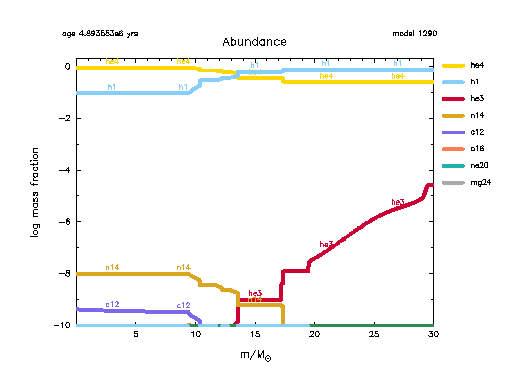
\includegraphics[scale=.7]{abund_001290}
\end{center}

Looking at \(m=12M_{\odot}\), where CNO and pp fusion are approximately equal, \(Z_{CNO}\approx Z_{N} \approx 10^{-9}\)


\end{document}

